\chapter{Geschäftswertbeitrag}
\label{Geschaeftswertbeitrag}

\section{Definition}
Der Geschäftswertbeitrag (GWB), im Englischen Economic Value Added (EVA), definiert einen Residualgewinn, welcher eine absolute Nettogröße eines Gewinns nach Abzug der Kapitalkosten für das eingesetze Gesamtkapital ergibt. Diese Kennzahl wurde in den 1990er Jahren in der Unternehmensberatung Stern Stewart entwickelt.\footnote{\cite{wikipedia-eva}} \footnote{\cite{controlling-eva}}

\section{Berechnung}

Der Geschäftswertbeitrag setzt sich aus drei Elementen zusammen: Dem operativen Gewinn nach Steuern (NOPAT - Net Operating Profit After Taxes), das betriebsnotwenige Vermögen (NOA - Net Operating Assets) und die gewichteten durchschnittlichen Kapitalkosten (WACC - Weighted Average Cost of Capital).\\
Der NOPAT ist der Teil, der Operativ entschieden wird. Hierbei geht es darum, dass man das Richtige machen möchte, beziehungsweise etwas besser machen. Die NOA bezieht sich auf eine Entscheidung basierend auf der Investition. Hierbei wird die Verbindlichkeit aus dem laufenden Geschäft nicht berücksichtig, ebenfalls das Ergebnis der Finanzierungstätigkeit. Zuletzt gibt es noch die Finanzierungsentscheidung, welches durch das WACC repräsentiert wird. Zudem kann das WAAC eine gesicherte Aussage über das Unternehmensrisiko geben.\footnote{\cite{bwllexicon-eva}} \footnote{\cite{wikipedia-eva}}\\
In folgender Abbildung \ref{fig:zsmgeschaeftswertbeitrag}\footnote{Quelle: \url{https://www.bwl-lexikon.de/app/uploads/economic-value-added.png}} sind die drei Bestandteile des Geschäftswertbeitrag im Zusammenhang grafisch dargestellt:

\begin{figure}[!h]
    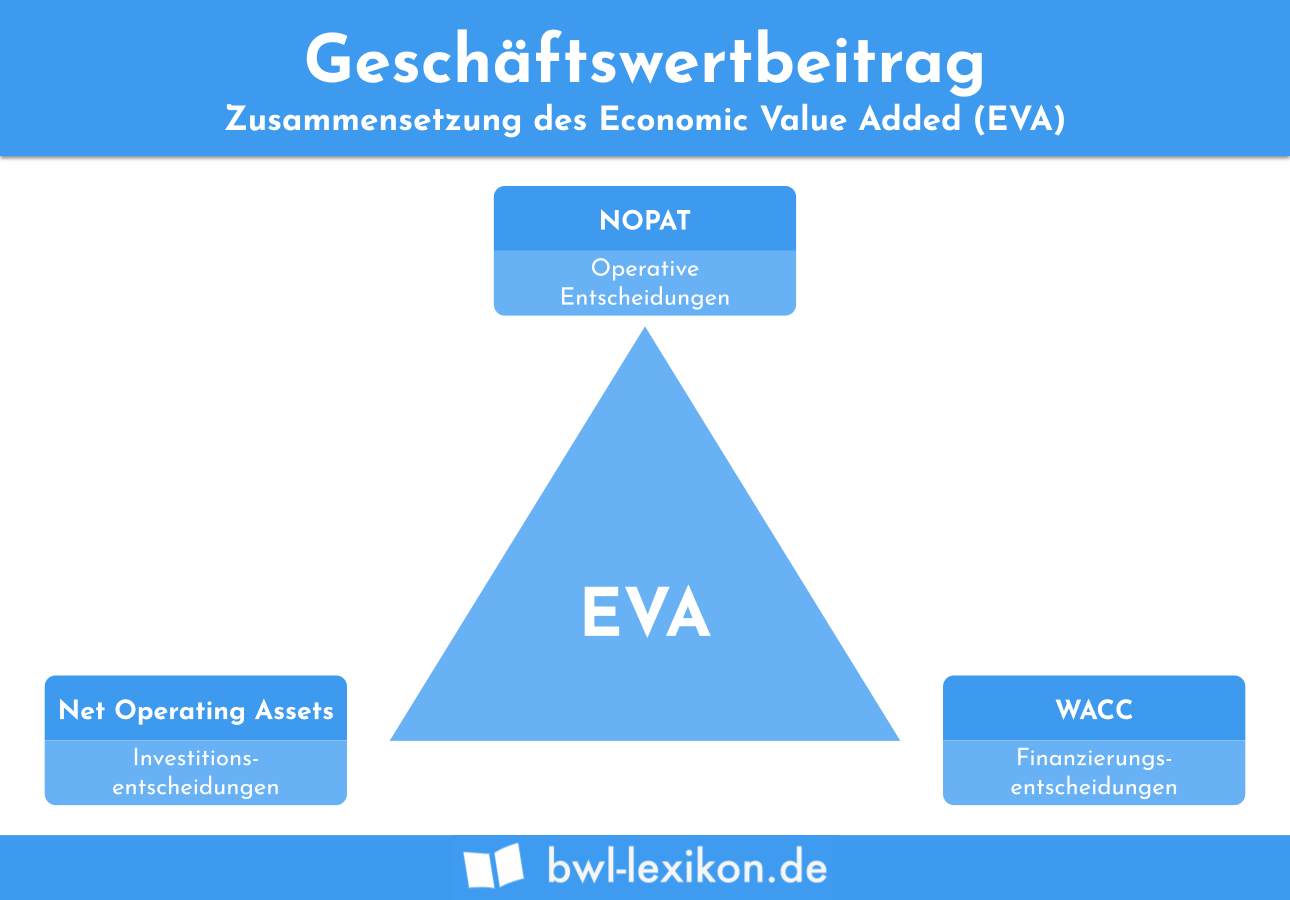
\includegraphics[width=\linewidth]{./media/economic-value-added.png}
    \caption{Zusammensetzung Geschäftswertbeitrag}
    \label{fig:zsmgeschaeftswertbeitrag}
\end{figure}

Es gibt zwei Methoden, um den GWB zu berechnen. Den subtraktiven Ansatz und den multiplikativen Ansatz. Beide Ansätze führen zum gleichen Berechnungsergebnis. Sie unterscheiden sich letztlich nur in der Fokussierung auf das absolute oder relative Erfolgsziel.

\subsection{Subtraktiver Ansatz}

Bei dem substraktiven Ansatz werden von dem operativen Jahresergebnis die durchschnittlichen Kapitalkosten mal dem betriebsnotwenigem Vermögen abgezogen. Folgende Formel \eqref{eq:subtraktiver-geschaeftswertbeitrag}\footnote{\cite{wikipedia-eva}} repräsentiert diese Rechnung:

\begin{equation}
    GWB = NOPAT - WACC \cdot NOA
    \label{eq:subtraktiver-geschaeftswertbeitrag}
\end{equation}

\subsection{Multiplikativer Ansatz}

Bei dem multiplikativen Ansatz werden von der (Ist-)Gesamtkapitalrendite (IRR - Internal Rate of Return) die durchschnittlichen Kapitalkosten abgezogen und auf dieses Ergebnis wird dann das betriebsnotwenige Vermögen multipliziert. Dies wird in folgender Formel \eqref{eq:mupliplikativ-gwb-geschaeftswertbeitrag}\footnote{\cite{wikipedia-eva}} dargestellt. In der Formel \eqref{eq:mupliplikativ-irr-geschaeftswertbeitrag}\footnote{\cite{controllingportal-eva}} wird die berechnung der IRR für die Vollständigkeit dargestellt. Die IRR berechnet sich aus dem Quotuenten aus dem operativen Gewinn nach Steuern und dem  betriebsnotwenigem Vermögen multipliziert mit 100.

\begin{equation}
    GWB = (IRR - WACC) \cdot NOA
    \label{eq:mupliplikativ-gwb-geschaeftswertbeitrag}
\end{equation}

\begin{equation}
    IRR = \frac{NOPAT}{NOA} \cdot 100
    \label{eq:mupliplikativ-irr-geschaeftswertbeitrag}
\end{equation}

\bigskip

\noindent
Vorraussetzung für diese Methode ist, dass das NOPAD immer größer als die Kapitalkosten, welche bei der Investition anfallen, ist.\footnote{\cite{bwllexicon-eva}}

\section{Beispielrechnung}

\subsection{Rechnung}

Da der Fokus auf der Berechnung des Geschäftswertbeitrags liegt, werdn für die Beispielrechnungen die Werte bereits angenommen. Demzufolge beträgt der WACC 8\%, der NOPAT beträgt 10000 € und die NOA belaufen sich auf 90000 €.

\subsubsection{Subtraktiver Ansatz}

Mit der Anwendung des substraktiven Ansatzes \eqref{eq:subtraktiver-geschaeftswertbeitrag} ergibt sich folgende Rechnung:

\bigskip
\noindent
GWB = 10000 € - 0,08 $\cdot$ 90000 € = 2800 €


\subsubsection{Multiplikativer Ansatz}

Da beide Ansätze das selbe Ergebnis haben sollten, sollte auch der multiplikative Ansatz \eqref{eq:mupliplikativ-gwb-geschaeftswertbeitrag} einen GWB von 2800 ergeben:

\bigskip
\noindent
GWB = (($\frac{10000}{90000})$ - 0,08) $\cdot$ 90000 € = 2800 €

\subsection{Interpretation}

Der Geschäftswertbeitrag von 2800 € zeigt, dass die Rendite über den Kosten für das eingesetze Kapital liegt, weshalb diese Investition durchaus durchführbar ist. Wäre der Wert negtaiv, würde die Investition verluste aufweisen und es wäre davon abzuraten, diese zu tätigen.

\section{Bewertung}

Der Geschäftswertbeitrag ist eine einfache Methode, um einen Betrag zu erhalten, wie sich eine Investition auswirkt. Jedoch ist die Berechnung an mehrere Faktoren gebunden, welche das Ergebnis sehr leicht verfälschen können. Auch die Entwicklung in der Zukunft ist durch den GWB nicht ersichtlich. Zuletzt lässt der Freiheitsgrad eines Unternehmens, anpassungen vorzunehmen, die Vergleichbarkeit unterschiedlicher Jahre verringert.\footnote{\cite{controlling-eva}}